% -*- root: rapport.tex -*-
\documentclass[a4paper, 12pt]{article}
\usepackage{graphicx}
\DeclareGraphicsExtensions{.pdf,.png,.jpg}
\usepackage{xcolor}   %May be necessary if you want to color links
\usepackage{hyperref}
\usepackage{mathtools}
\usepackage{listings}
\usepackage{pgfplots}
\usepackage{pgfplotstable}
\usepackage{booktabs}
%\usepackage{inconsolata}




\hypersetup{
    colorlinks=true, %set true if you want colored links
    linktoc=all,     %set to all if you want both sections and subsections linked
    citecolor=black,
    filecolor=black,
    linkcolor=black,
    urlcolor=blue
}

\lstdefinestyle{customc}{
  belowcaptionskip=1\baselineskip,
  breaklines=true,
  frame=single,
  language=C,
  showstringspaces=false,
  basicstyle=\footnotesize\ttfamily,
  keywordstyle=\bfseries\color{green!40!black},
  commentstyle=\itshape\color{purple!40!black},
  identifierstyle=\color{blue},
  stringstyle=\color{orange},
  tabsize=4
}
\lstset{escapechar=@,style=customc}

\title{Utilizing Amazon's Zookeeper to handle scaling and maintenance of a Voldemort cluster}
\author{Eivind Siqveland Larsen and Knut Nygaard,\\
        Department of Computer Science,\\
        NTNU,
        Trondheim}

\begin{document}
\maketitle
\thispagestyle{empty}

\clearpage

\begin{abstract}
NoSQL databases often support scalability and high availability.
We address Voldemort, which is a popular, highly available NoSQL database that can be run on several nodes.
The system is cumbersome to setup and maintain. As clusters grow in size, scaling into hundreds of nodes, management and administrative tasks become increasingly complex. We have therefore focused on automating management of a running cluster of nodes.

We have migrated the configuration storage of the Voldemort distributed NoSQL database from local XML files on disk to global objects using Apache ZooKeeper.

Using native tools and ZooKeeper coordination, we have implemented a fault tolerant, redundant service. The service manages node discovery, configuration generation and propagation. It also has components for live monitoring and adjustment of responsibility to match each nodes available system resources.

\end{abstract}

\clearpage
\renewcommand{\abstractname}{Sammendrag}
\begin{abstract}
Vi har flyttet konfigurasjon av en distribuert NoSql database fra lokalt lagrede XML filer til globalt tilgjengelige objekter ved hjelp av Apache ZooKeeper.

Vi har brukt ZooKeepers egenskaper for koordinasjon og andre verktøy til å implementere en feiltolerant, redundant tjeneste for å ta hånd om nye noder, generere konfigurasjonsfiler, propagere endringer og automatisk tilpassing av det kjørende systemet til den enkelte nodes tilgjengelige systemressurser.
\end{abstract}


\begin{aknowledgements}
We would like to than Svein Erik Bratsberg for his guidance and assistance in the project.
We would also like to thank LinkedIn for creating and publishing their take on Dynamo and making it open source.
\end{aknowledgements}

\setcounter{page}{1}
% introduction.tex

\section{Introduction}
This section explains the background for our project, what goals we have and what methods we have employed to reach our goals. 

Section \ref{sec:technical_background} explains technology and techniques commonly used in distributed systems.

TODO: INTRODUCE OTHER SECTIONS AND CHAPTERS

\subsection{WHAT}
Short what and why.

We have chosen to work with Voldemort, which is an open source implementation of Amazon’s Dynamo. 


\subsection{Background}
Traditional relational database systems are generally very safe to use, usually providing all of the ACID (\emph{Atomicity, Consistency, Isolation, Durability}) properties.
This guarantees that all committed transactions are processed reliably. 
Today a lot of services needs to support up to millions of users and serve thousands of requests per second, but experience has shown that databases providing ACID guarantees have trouble scaling. 
To allow for cost effective scaling commodity hardware is used instead of expensive specialized servers. To continue scaling by adding numerous small servers, applications need to become increasingly distributed.

The main reason for ACID databases having troubles scaling is the strong guarantees of atomic operations, isolation and consistency. 
To allow for atomic operations in a distributed systems a distributed commit log would be required. 
Similarly to guarantee isolation distributed locks would be required. In a system with thousands of concurrent users lock contention can become a serious issue. 
Lastly to guarantee consistency across multiple machines requires significant overhead with regards to keeping all replicas consistent. 

Distributed NoSQL databases often sacrifice consistency and isolation requirements to achieve higher availability with satisfactory durability. These systems often provide a highly available service and eventual consistency.
The databases are designed to scale linearly, however managing and scaling these systems are not always trivial\cite{tellybug}. 


\subsection{Voldemort and Dynamo}
Voldemort is a distributed key-value storage system based off Amazon's paper on Dynamo, Amazons's highly available key-value store. Voldemort was created by LinkedIn and the first public release was in 2009. It is still under development. Voldemort supports a simple set of operations limited to put, get and delete. Stored objects are uniquely identified by a key and are considered by the system as binary blobs. Voldemort is commonly used for storing lots of smaller objects, typically less than 1MB.  As with other NoSQL implementations, Voldemort sacrifices consistency and isolation requirements to achieve higher availability with satisfactory durability. In fact, we will later see that most of this behavior is easily tunable and left as design choices per implementation.

Compared with Apaches Cassandra, Voldemort lacks the power of column families and multi-key lookup. This means that any application powered by Voldemort requires addtional logic to handle more advanced queries. For simple read heavy workloads however, Voldemort is blazingly fast serving over 20 000 read requests per second per node. 

Voldemort is currently being used by a number of known companies. At LinkedIn they use Voldemort both as read-only and read-write stores. Services powered include LinkedIn Search, news and Who viewed your profile. At Ebay they use Voldemort as a read-only store for distributed lookups, and the dating site eHarmony uses Voldemort as a high volume read/write store.

There are several factors that was important for us when choosing which distributed key-value store to work with. We both had detailed theoretical knowledge of Dynamo after holding a presentation on their paper. The simple design and data model of Voldemort also was a good fit for our project as we did not have any application specific requirements for our storage system to meet. Lastly we wanted to work with an open source project. Voldemort fulfilled all these requirements. 

Voldemort keep its configuration data in several XML files. These files reside on each individual node in the cluster. The process of executing a repartition or rebalance involves another set of xml files as well as various scripts that must be run. As the number of nodes grows this number of configuration files can get out of hand quickly. 
As a result, creating a system to handle these configuration files was proposed as a ``fun project'' on the project-voldemort website. Apache ZooKeeper was proposed as a possible service for this system.  


\subsection{Goals}
We have chosen to implement this proposed configuration system by moving Voldemort's configuration data into ZooKeeper. In addition we would like to utilize the powerful features of ZooKeeper to create an automated service for managing a running Voldemort cluster. 

% Create a system for automatically including new nodes in a set of member nodes.
% For Voldemort, this includes redistributing partitions and updating routing information without making the system unresponsive, i.e. without incurring downtime.

In short our goals are the following:

\begin{enumerate}
	\item{Move Voldemort configuration data away from each local node and into ZooKeeper}
	\item{Simplify the rebalance process using ZooKeeper}
	\item{Create a service for automatic management of the cluster, including node discovery, membership and rebalancing with new members}
	\item{Create a monitor service to monitor live nodes}
\end{enumerate}

\subsection{Method}
We plan to use virtual machines as our cluster nodes. This greatly simplifies setup of environments and scaling, but is not ideal for performance. We will rewrite the MetadataStore in Voldemort to utilize ZooKeeper instead of local files. As ZooKeeper does not offer advanced primitives, we need to write the ones we need. Finally we will create a service for node discovery, membership and automatic management. The monitor service will act as decision support system for this automated service. 


% The supported queries are limited to simple get and put operations on objects uniquely identified by a key. 
% The objects stored are by the system considered binary blobs.
% The database is mainly used to store lots of smaller items, typically less than 1MB in size.

% Voldemort and Dynamo sacrifices consistency and isolation requirements to achieve higher availability with satisfactory durability.
% In fact, we will later see that most of this behavior is easily tunable and left as design choices per implementation.
% You should also note Voldemort (and Dynamo) does not guarantee any form of isolation and does not support multiple key updates.


%\subsubsection{Motivation for these systems}
%Traditional relational database systems are generally very safe to use, usually providing all of the ACID (\emph{Atomicity, Consistency, Isolation, Durability}) properties.
%This guarantees that all committed transactions are processed reliably.
%Experience has however shown that databases providing ACID guarantees have trouble scaling. It is very difficult, if not impossible, to have ACID databases handle the high traffic volumes in addition to the high availability demands of today.

%Voldemort and Dynamo sacrifices consistency and isolation requirements to achieve higher availability with satisfactory durability.
%In fact, we will later see that most of this behavior is easily tunable and left as design choices per implementation.
%You should also note Voldemort (and Dynamo) does not guarantee any form of isolation and does not support multiple key updates.




\clearpage
\tableofcontents

\clearpage
\listoffigures

\clearpage

\section{Hardware}
\label{sec:hardware}

\subsection{Mac Mini}
We server running voldemort is a a Mac Mini Mid 2010 model. It has a Intel Core Duo 2.4 GHz processor, 8 GBs of RAM and solid state storage. We run the latest OS X 10.9.1

\begin{figure}[h]
    \centering
    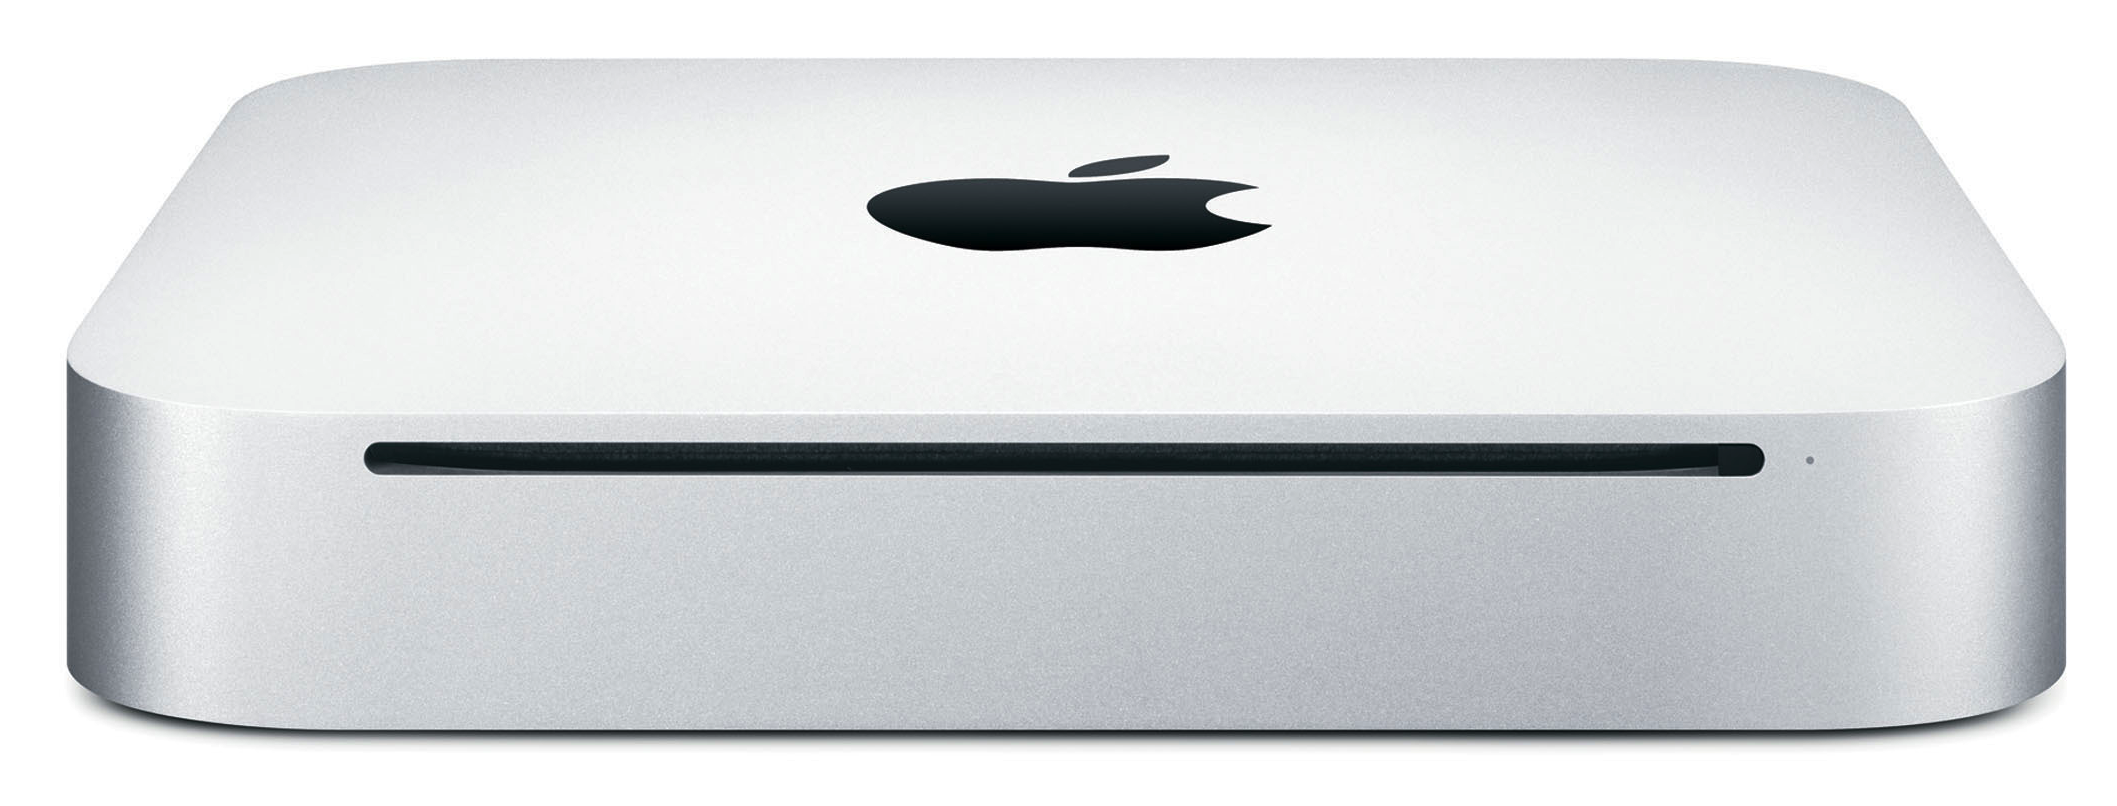
\includegraphics[width=0.8\textwidth]{hardware/mac-mini-06-2010}
    \caption{Mac Mini 2010}
    \label{fig:macmini_hw}
\end{figure}



\clearpage
\bibliographystyle{plain}
\bibliography{references}

\end{document}
